
\section{Criterio de validación}

La verificación funcional se organizó de acuerdo con los niveles del diseño.
Primero se probaron los bloques elementales de forma aislada. Luego se
verificaron el núcleo UART y el controlador. Por último, se comprobó el
recorrido completo entre los pines de recepción y transmisión. Este orden
permitió revisar cada función antes de evaluar la integración del sistema.

Todos los bancos de pruebas son autocheckeables. Cada uno genera sus estímulos y
determina el valor esperado mediante un modelo independiente o una secuencia
dirigida. Después compara ese valor con la salida del diseño mediante una
desigualdad estricta. Si encuentra una diferencia, incrementa el contador de
errores y finaliza la simulación con \texttt{\$fatal}.

Cada banco incorpora también un watchdog que limita la duración de la
simulación. Si el diseño queda esperando indefinidamente, el banco informa el
error en lugar de considerar que la prueba terminó correctamente.

El resultado PASS confirma que el banco terminó sin diferencias, pero no indica
por sí solo qué comportamiento fue comprobado. Por eso, cada resultado se
relaciona con los estímulos aplicados y con las señales observadas.

La tabla~\ref{tab:trazabilidad} relaciona cada requisito con el banco que lo
verifica y con la evidencia obtenida. Las formas de onda incluidas más adelante
muestran las señales necesarias para seguir los estímulos y las respuestas. Los
casos restantes se comprueban mediante las comparaciones automáticas de cada
banco. En cada nivel se presentan el criterio utilizado, el resultado observado
y la interpretación de esos resultados.

\begin{table}[H]
	\centering
	\small
	\begin{tabularx}{\textwidth}{L{3.3cm}L{3.8cm}Y}
		\toprule
		\textbf{Requisito} & \textbf{Banco} & \textbf{Evidencia} \\
		\midrule
		Conservar la ALU & \texttt{alu\_tb} & 814 comparaciones y ocho operaciones. \\
		Tick periódico & \texttt{baud\_tick\_gen\_tb} & Intervalo exacto y reset. \\
		Buffer ordenado & \texttt{fifo\_tb} & Lleno, vacío, bloqueo y wrap-around. \\
		Recibir 8N1 & \texttt{uart\_rx\_tb} & Bytes, falso start y stop inválido. \\
		Transmitir 8N1 & \texttt{uart\_tx\_tb} & Orden LSB, duración y
		finalización. \\
		Integrar UART/FIFO & \texttt{uart\_core\_tb} & Ráfagas, orden y overrun. \\
		Interpretar la terna & \texttt{alu\_uart\_}\newline\texttt{controller\_tb} &
		EXECUTE, timeout, error RX y backpressure. \\
		Recorrido pin a pin & \texttt{alu\_uart\_top\_tb} &
		812 transacciones, reset, recuperación y LED. \\
		\bottomrule
	\end{tabularx}
	\caption{Trazabilidad entre requisitos y bancos de pruebas.}%
	\label{tab:trazabilidad}
\end{table}

\section{Bloques elementales: ALU, temporización, FIFO y UART}

El primer nivel de verificación estudia por separado los bloques que realizan
las funciones básicas del sistema. De esta manera se puede comprobar el cálculo
de la ALU, la generación de los ticks, el comportamiento del FIFO y la
formación de las tramas UART antes de conectarlos entre sí.

\subsection{Criterio y estímulos}

El archivo \texttt{tb/alu\_tb.sv} verifica que la ALU conserve el
comportamiento definido para sus ocho operaciones. El banco aplica catorce
casos dirigidos y cien pares pseudoaleatorios por cada operación. La secuencia
aleatoria utiliza la semilla fija \texttt{32'h1a2b3c4d} para que pueda
repetirse.

El modelo de referencia calcula el resultado y las banderas carry y overflow
con expresiones diferentes de las utilizadas por el DUT. La bandera Z se
obtiene a partir del resultado esperado. En total, el banco realiza 814
comparaciones.

La prueba del generador se encuentra en
\texttt{tb/baud\_tick\_gen\_tb.sv}. Para reducir el tiempo de simulación se
utilizan una frecuencia de \SI{1000}{\hertz}, una velocidad de \num{25} baud
y un sobremuestreo 4x. Estos valores mantienen el divisor en diez y permiten
comprobar tres intervalos completos en pocos ciclos. El banco también activa el
reset y verifica que no se produzca ningún pulso espurio.

El archivo \texttt{tb/fifo\_tb.sv} comprueba el orden de los datos y el
comportamiento de la cola en sus límites. Primero escribe los valores
\texttt{11}, \texttt{22}, \texttt{33} y \texttt{44} hasta completar las
cuatro posiciones. A continuación intenta escribir \texttt{99} y comprueba que
el dato sea rechazado.

Después de retirar parte del contenido, el banco escribe \texttt{55} y
\texttt{66}. Con esta secuencia obliga a los punteros a volver al comienzo de
la memoria. También aplica una lectura y una escritura durante el mismo ciclo
con el FIFO lleno. Cada dato extraído se compara con el orden en que fue
insertado.

La recepción se verifica mediante
\texttt{tb/uart\allowbreak\_rx\allowbreak\_tb.sv}. El banco envía
las tramas correspondientes a \texttt{00}, \texttt{FF}, \texttt{A5} y
\texttt{3C}. Luego mantiene la entrada en bajo durante cuatro ticks para
producir un falso start. También envía una trama cuyo bit de stop permanece en
bajo. Después de estos errores transmite \texttt{69} para comprobar que el
receptor pueda volver a aceptar una trama válida.

El archivo \texttt{tb/uart\_tx\_tb.sv} verifica el recorrido opuesto. El
transmisor recibe los bytes \texttt{A5}, \texttt{00} y \texttt{FF}. El banco
observa la línea durante las dieciséis muestras de cada bit, comprueba que D0 se
envíe primero y exige un único pulso de finalización por cada trama.

\subsection{Resultado observado}

La figura~\ref{fig:wave-rx-a5} muestra la recepción del byte \texttt{A5}. La
línea serie presenta primero el bit de start y luego los ocho bits de datos.
Durante ese intervalo, la FSM permanece en DATA y
\texttt{bit\_count} avanza con cada muestra aceptada. El registro interno
reconstruye el byte mediante desplazamientos. El pulso \texttt{done} aparece
recién después de comprobar el bit de stop y el valor publicado es
\texttt{A5}.

\begin{figure}[H]
	\centering
	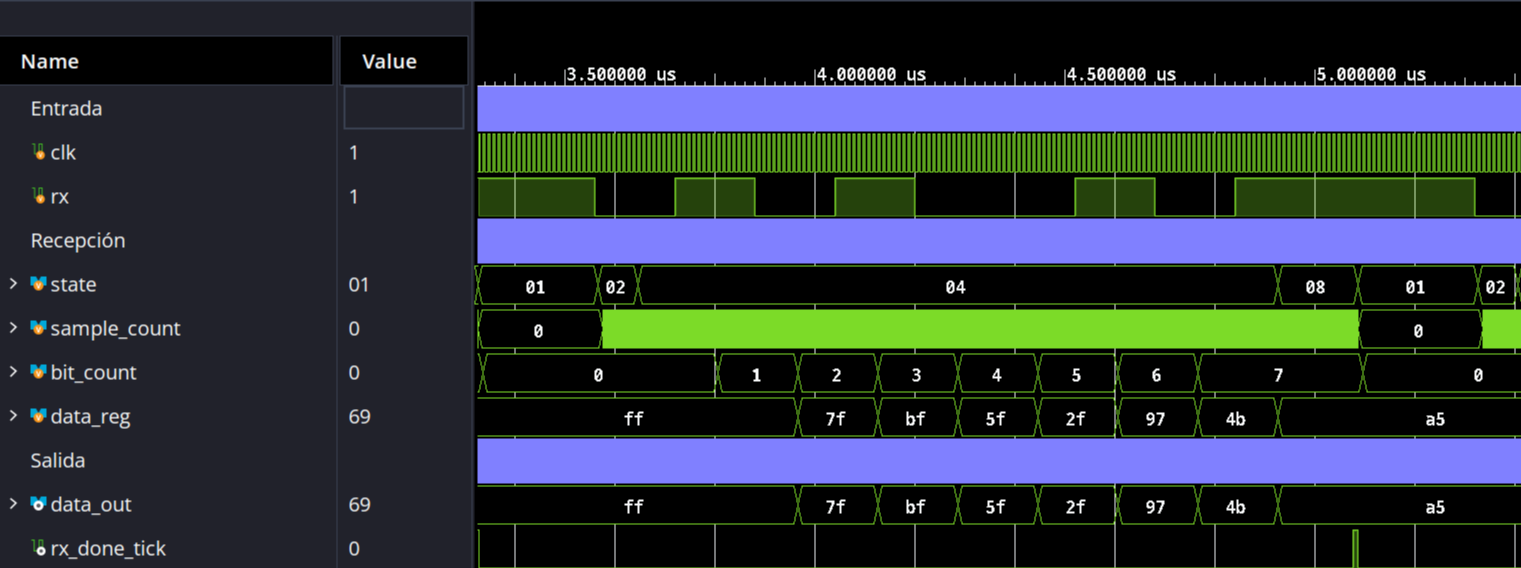
\includegraphics[width=\textwidth]{img/vivado_wave_uart_rx_a5.png}
	\caption{Recepción válida de \texttt{A5} en \texttt{uart\_rx\_tb}.}%
	\label{fig:wave-rx-a5}
\end{figure}

La figura~\ref{fig:wave-rx-errors} reúne las dos tramas defectuosas. El pulso
breve de la entrada produce el primer \texttt{frame\_error}. La trama
siguiente alcanza el estado DATA, pero el nivel bajo durante el stop produce el
segundo error. En ninguno de los casos se activa \texttt{done}.

Después de detectar cada defecto, el estado RECOVER espera que la entrada RX
regrese al nivel alto antes de volver a IDLE. Por esta razón, cada trama
defectuosa genera un solo pulso de error.

\begin{figure}[H]
	\centering
	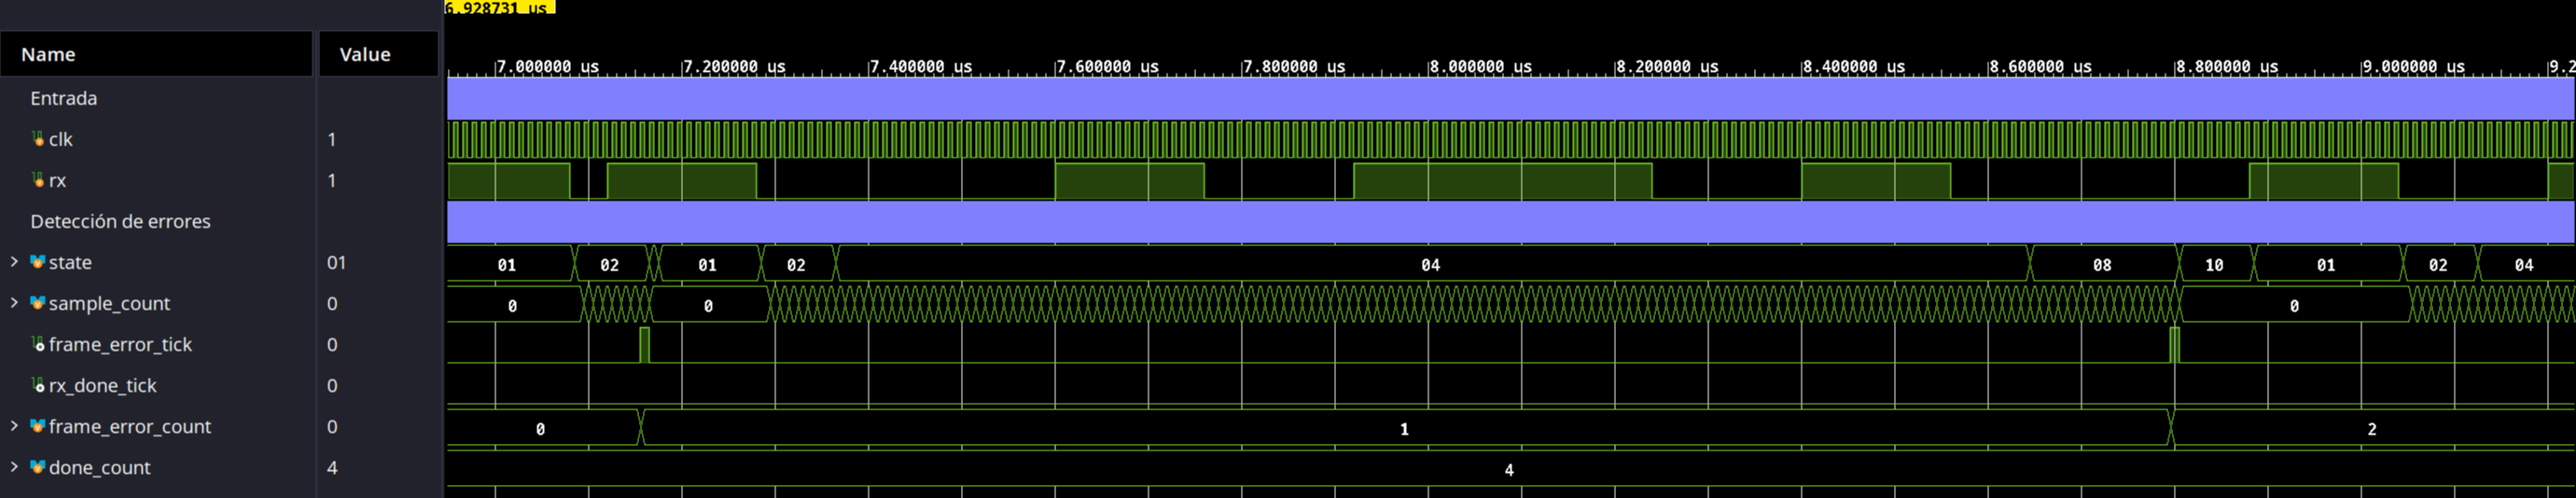
\includegraphics[width=\textwidth]{img/vivado_wave_uart_rx_errors.png}
	\caption{Detección de falso start y stop inválido en \texttt{uart\_rx\_tb}.}%
	\label{fig:wave-rx-errors}
\end{figure}

La figura~\ref{fig:wave-tx-a5} presenta la transmisión de
\texttt{A5 = 1010\,0101}. Después del start en nivel bajo, la línea muestra la
secuencia 1, 0, 1, 0, 0, 1, 0, 1. Este orden corresponde al envío desde D0 hasta
D7. La señal \texttt{busy} permanece activa durante toda la trama y
\texttt{done} se mantiene en alto durante un solo ciclo después del stop.

\begin{figure}[H]
	\centering
	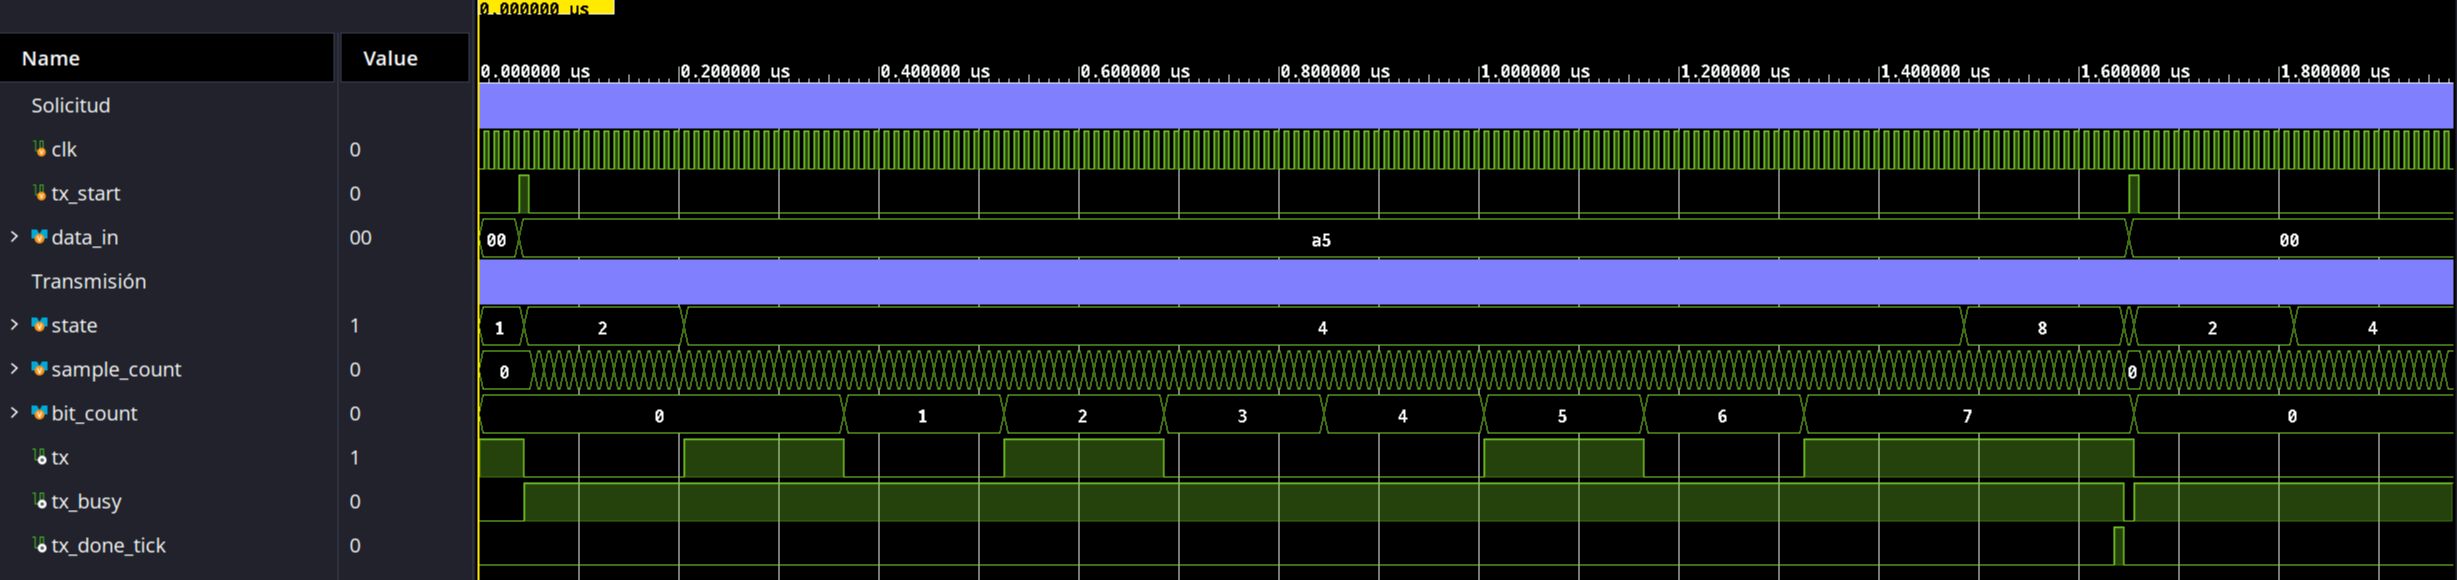
\includegraphics[width=\textwidth]{img/vivado_wave_uart_tx_a5.png}
	\caption{Serialización de \texttt{A5} en \texttt{uart\_tx\_tb}.}%
	\label{fig:wave-tx-a5}
\end{figure}

La figura~\ref{fig:wave-fifo} muestra la ocupación completa del FIFO. El
contador alcanza el valor cuatro y activa \texttt{full}. El intento de
escribir \texttt{99} no modifica el dato ubicado en la cabeza de la cola.

Las escrituras posteriores reutilizan las posiciones liberadas, pero no alteran
el orden de lectura. La secuencia observada es
\texttt{11,22,33,44,55,66,77,88}. Al retirar el último dato, el contador vuelve
a cero y se activa \texttt{empty}.

\begin{figure}[H]
	\centering
	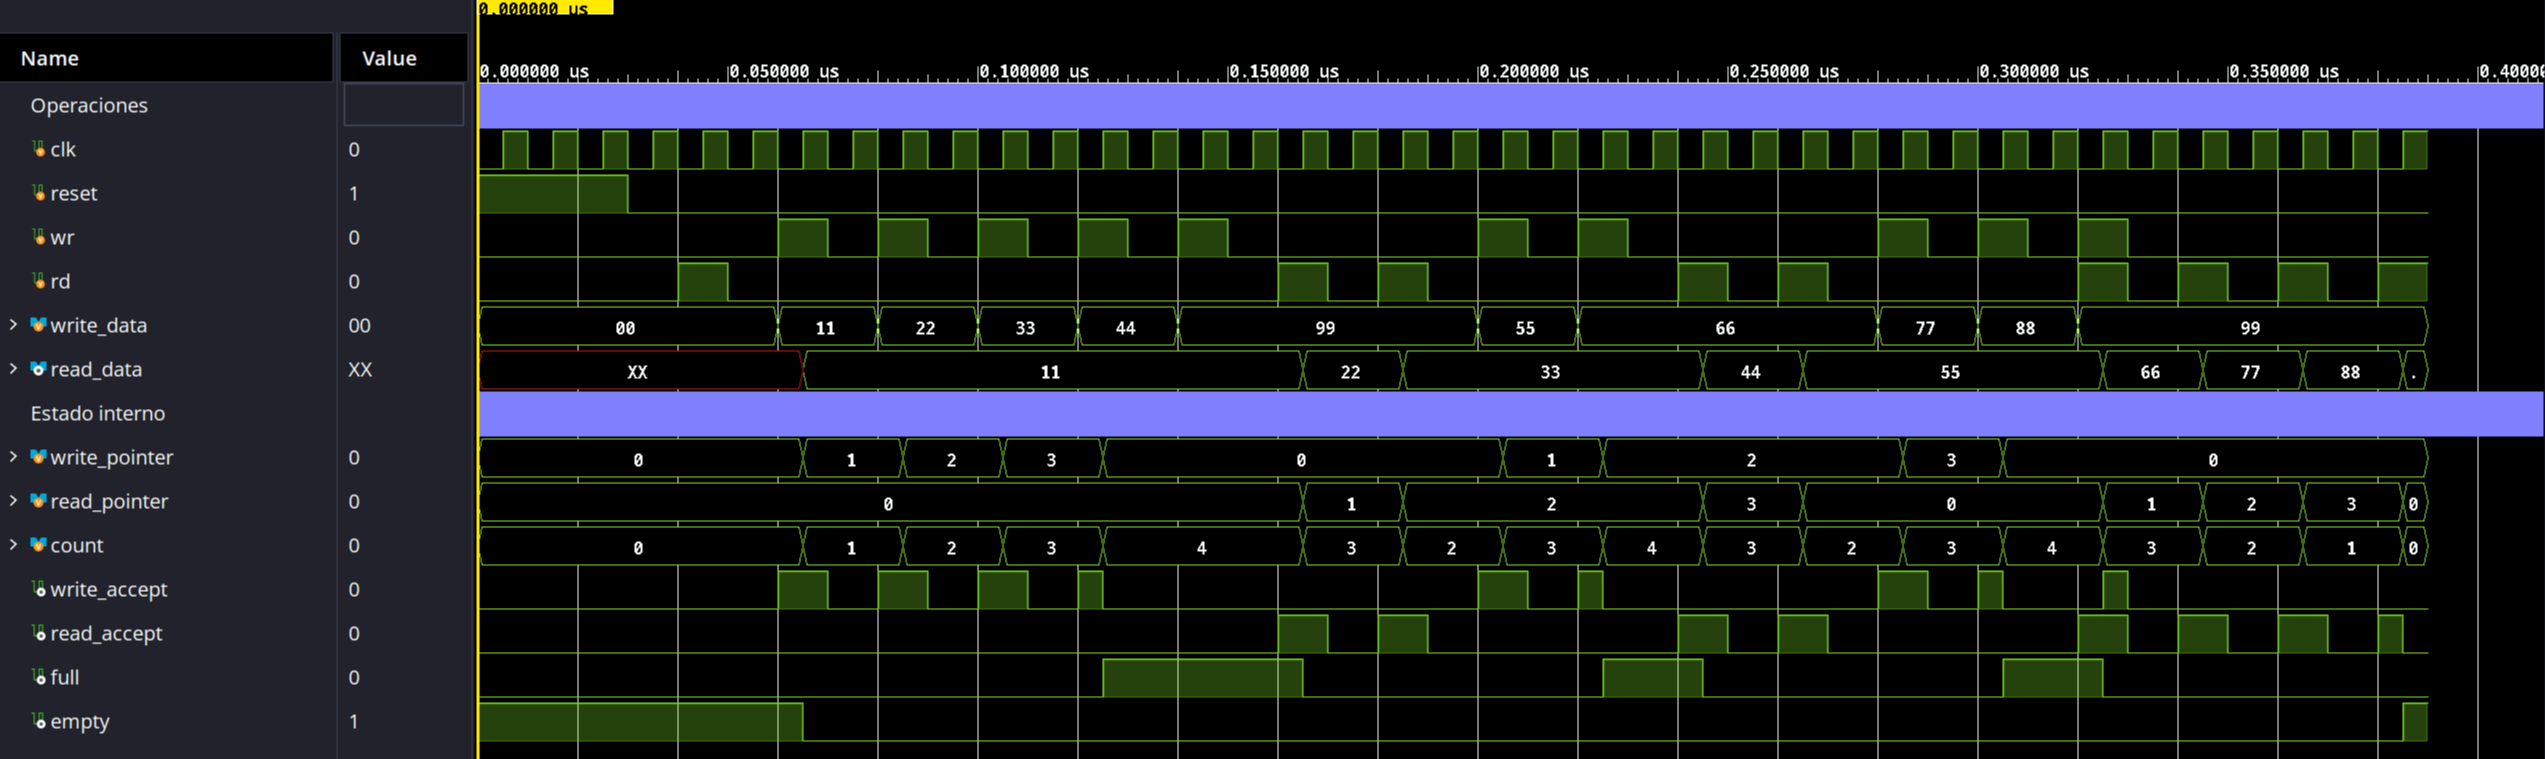
\includegraphics[width=\textwidth]{img/vivado_wave_fifo.png}
	\caption{Límites, accesos simultáneos y wrap-around en \texttt{fifo\_tb}.}%
	\label{fig:wave-fifo}
\end{figure}

\subsection{Interpretación}

Los cuatro bancos elementales finalizaron con el resultado PASS. Las 814
comparaciones de \texttt{alu\_tb.sv} confirmaron que la integración no
modificó el comportamiento de la ALU. La prueba de
\texttt{baud\_tick\_gen\_tb.sv} comprobó la periodicidad con la
parametrización reducida y utilizó la misma expresión del divisor que el
diseño. Este ensayo no mide la precisión del oscilador físico.

Las capturas del receptor y del transmisor muestran el recorrido completo del
byte \texttt{A5}. En ellas se puede seguir el orden de los bits y el cambio de
estado que ocurre durante cada parte de la trama. Los demás bytes no se
incluyeron en las figuras, pero fueron comprobados automáticamente por sus
respectivos bancos.

El archivo \texttt{fifo\_tb.sv} verificó que los datos se retiraran en el mismo
orden en que habían sido escritos. También comprobó que \texttt{full} se
activara al ocupar las cuatro posiciones y que \texttt{empty} lo hiciera
después de retirar el último dato.

Estas pruebas confirman el funcionamiento individual de los bloques. Todavía no
comprueban que el controlador pueda recibir una solicitud completa ni que el
resultado recorra todo el camino entre ambos pines UART.

\section{Subsistemas: núcleo UART y controlador}

Una vez verificados los bloques elementales, se probaron las dos partes que
coordinan el intercambio. El núcleo UART reúne el receptor, el transmisor y las
dos colas. El controlador interpreta los bytes recibidos y genera la respuesta
de la ALU. Los bancos de este nivel permiten revisar esas funciones sin
incorporar todavía el recorrido completo por las líneas serie.

\subsection{Criterio y estímulos}

El archivo \texttt{tb/uart\_core\_tb.sv} verifica primero el camino de
recepción. Para ello envía cinco bytes consecutivos sobre RX sin retirar ningún
dato. Los primeros cuatro deben permanecer almacenados en el FIFO. La llegada
del quinto debe generar exactamente un overrun. Después, el banco retira los
cuatro bytes y comprueba que mantengan el orden de llegada.

El mismo banco verifica luego el camino de transmisión. En este caso escribe
\texttt{A5}, \texttt{00}, \texttt{FF} y \texttt{3C} en la cola
correspondiente. Un decodificador implementado en el banco reconstruye las
cuatro tramas observadas sobre TX y compara los bytes obtenidos.

La prueba del controlador se encuentra en
\texttt{tb/alu\allowbreak\_uart\allowbreak\_controller\allowbreak\_tb.sv}. Este banco entrega y retira bytes a
través de la interfaz de los FIFO. De este modo puede comprobar la
interpretación de la secuencia A--B--opcode sin incluir los tiempos propios de
la transmisión UART.

Los casos dirigidos incluyen una suma normal, una suma con carry y otra con
overflow. También verifican SRA, AND, SUB, NOR, un opcode inválido y un opcode
con los bits superiores reservados. Para comprobar la espera de la salida, el
banco mantiene \texttt{tx\_full} activo durante cinco ciclos. Por último, deja
vencer el timeout de una operación incompleta y aplica
\texttt{rx\_error\_tick} después de recibir el operando A.

\subsection{Resultado observado}

La figura~\ref{fig:wave-controller} permite seguir primero la operación
\texttt{7F 01 20}. En la parte superior aparecen los tres bytes de la solicitud
sobre \texttt{r\_data}. Cada vez que hay un byte disponible, el controlador
activa \texttt{rd\_uart} para retirarlo de la cola de recepción. Las tres
lecturas almacenan el operando A, el operando B y el opcode. Al mismo tiempo, el
estado avanza por WAIT\_A, WAIT\_B y WAIT\_OPCODE.

Después de recibir el opcode, el controlador pasa a EXECUTE. El pulso
\texttt{capture\_result} registra el resultado \texttt{80} y las banderas de
la ALU. En ese momento, \texttt{result\_reg} toma el valor \texttt{80} y los
LED cambian a \texttt{480}. Los tres bits superiores de este patrón indican
que la bandera V está activa. Como la cola de transmisión tiene espacio,
\texttt{w\_data} presenta el resultado y \texttt{wr\_uart} genera el pulso
que lo escribe en el FIFO.

La parte derecha de la captura muestra una situación diferente con la operación
\texttt{0C 0A 24}. El controlador recibe los tres bytes y calcula el resultado
\texttt{C0}, pero \texttt{tx\_full} se encuentra en alto. Por esta razón,
permanece en WAIT\_TX y conserva la respuesta en \texttt{result\_reg}. Durante
esa espera, \texttt{wr\_uart} permanece en bajo y el resultado no se escribe
en una cola que ya está llena.

Cuando \texttt{tx\_full} vuelve a cero, el controlador genera el pulso de
escritura y entrega la respuesta pendiente. Recién entonces regresa a WAIT\_A
para comenzar una nueva solicitud. Esta parte de la figura muestra que una
demora en la transmisión no provoca la pérdida del resultado calculado.

\begin{figure}[H]
	\centering
	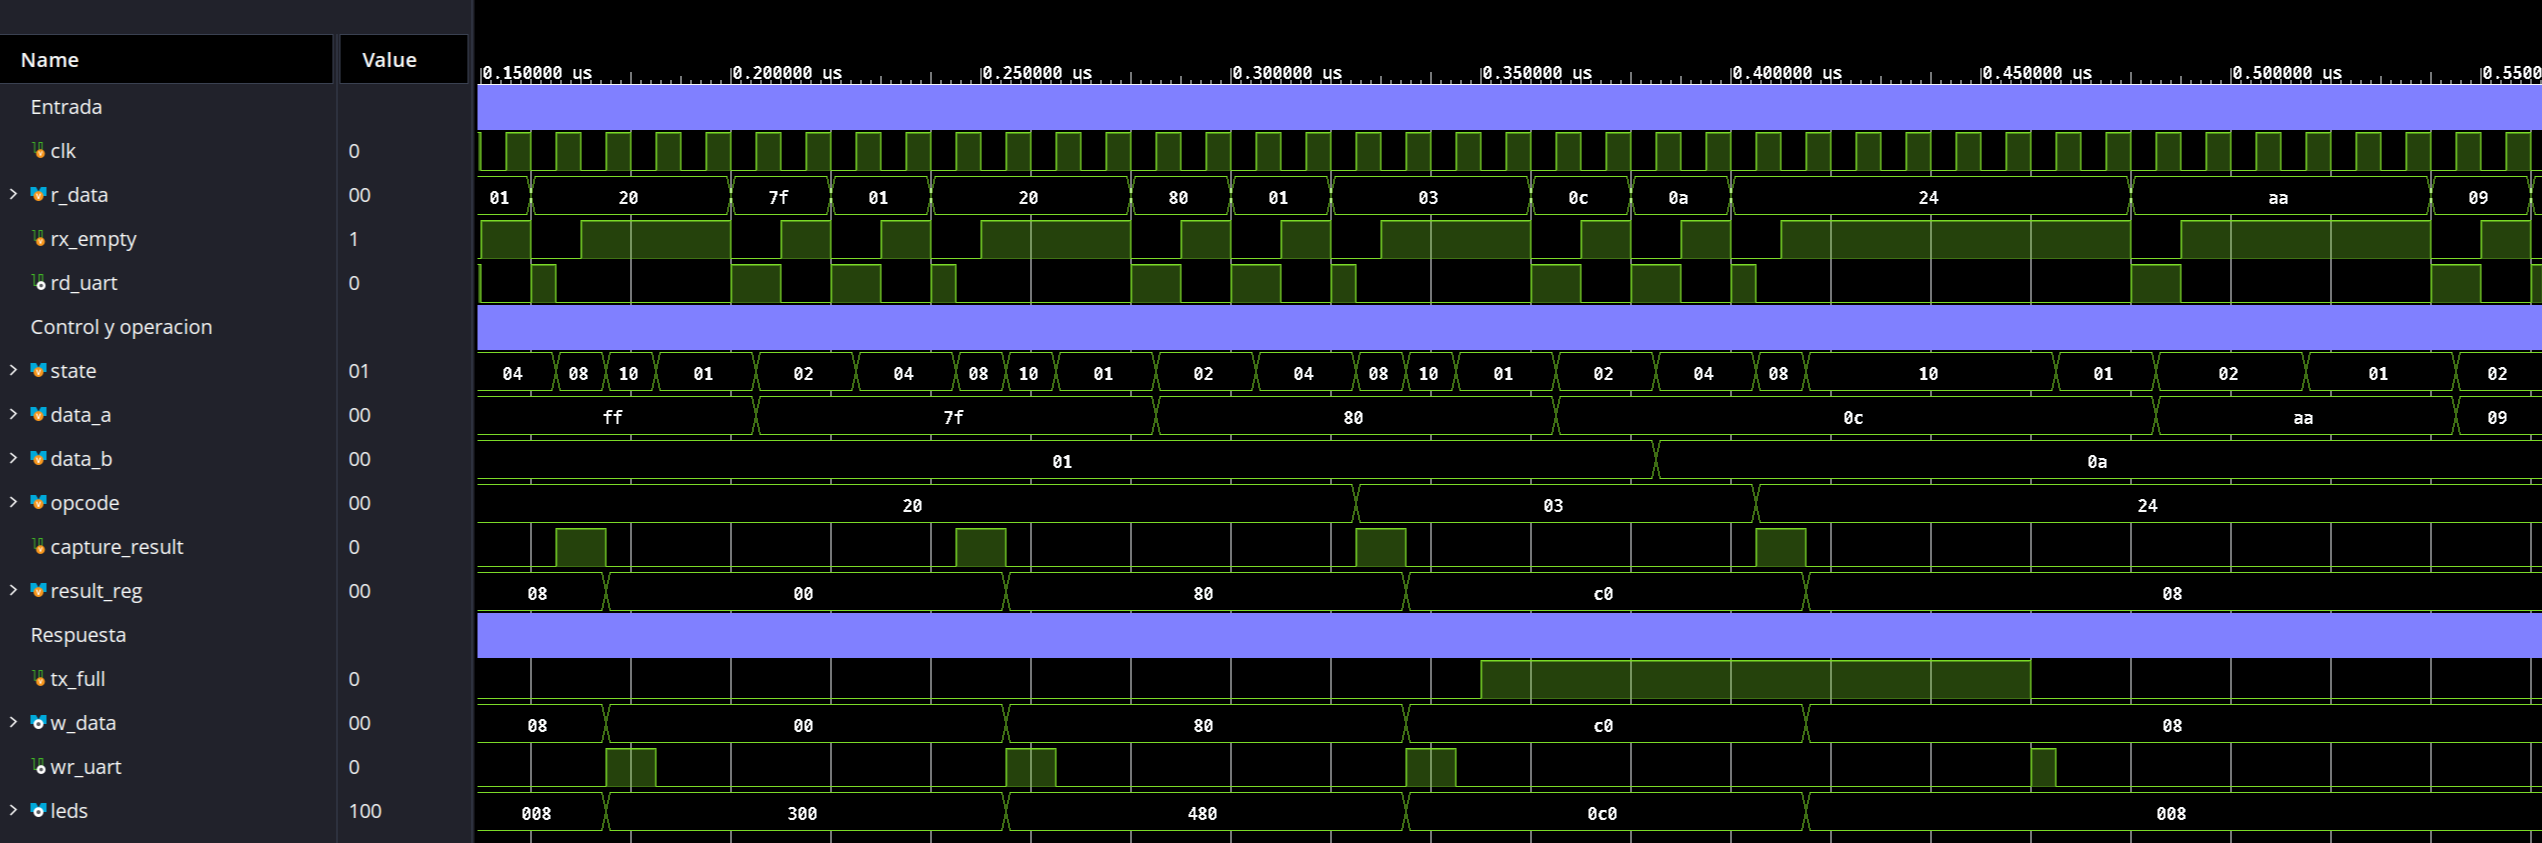
\includegraphics[width=\textwidth]{img/vivado_wave_controller.png}
	\caption{Operación y espera por capacidad en
	\texttt{alu\_uart\_controller\_tb}.}%
	\label{fig:wave-controller}
\end{figure}

XSim informó
\texttt{PASS: UART core FIFOs, overrun and serialized output} al finalizar el
banco del núcleo. Para el controlador informó
\texttt{PASS: ALU/UART controller protocol, stalls and recovery}. Ninguno de
los bancos produjo errores fatales ni alcanzó el límite de su watchdog.

\subsection{Interpretación}

El banco del núcleo confirmó que las colas conservan el orden de los bytes. La
prueba de recepción completa mostró además que un dato adicional produce un
error de overrun en lugar de sobrescribir el elemento más antiguo.

El banco del controlador confirmó que una respuesta permanece registrada
mientras la cola de transmisión está llena. También verificó que EXECUTE separa
la captura del opcode del registro del resultado. Los casos de timeout y error
de recepción mostraron que una solicitud incompleta se descarta antes de
aceptar una nueva.

En estas pruebas, uno de los extremos todavía es reemplazado por el propio banco.
El núcleo UART no está conectado a la ALU y el controlador recibe bytes
completos sin atravesar el receptor. Por lo tanto, los resultados de este nivel
no sustituyen una prueba del sistema integrado.

\section{Verificación extremo a extremo}

El último nivel comprueba el funcionamiento del módulo superior. En esta prueba
los estímulos ingresan como bits por \texttt{serial\_rx}. La respuesta también
se observa como una trama completa sobre \texttt{serial\_tx}. De esta manera
se incluye el mismo recorrido que utiliza una operación dentro de la FPGA.

\subsection{Criterio y estímulos}

El archivo \texttt{tb/alu\_uart\_top\_tb.sv} instancia el sincronizador, el
generador de ticks, el receptor, el transmisor, los dos FIFO, el controlador y
la ALU. Para conservar las relaciones temporales y reducir el costo de la
simulación, utiliza un reloj de \SI{100}{\kilo\hertz}, una velocidad de
\num{2500} baud y un sobremuestreo 4x. Con estos parámetros, el divisor
permanece en diez y cada bit dura cuarenta ciclos.

El banco no fuerza ninguna señal interna. Los estímulos modifican únicamente
\texttt{serial\_rx} y la respuesta se reconstruye a partir de
\texttt{serial\_tx}.

Los primeros doce casos son dirigidos. En las operaciones válidas se incluyen
una suma normal, una suma con carry, una suma con overflow, SUB, SRA, SRL y NOR.
También se comprueban un opcode inválido y un opcode con los bits superiores
reservados.

Los tres casos restantes se concentran en la recuperación. El primero envía un
byte aislado y espera que venza el timeout. El segundo introduce un bit de stop
inválido y luego transmite una operación correcta. El tercero activa el reset
durante una trama.

Después de los casos dirigidos, el banco aplica cien pares pseudoaleatorios para
cada una de las ocho operaciones. La secuencia utiliza la semilla
\texttt{32'h1a2b3c4d}. En total se ejecutan 800 operaciones aleatorias y 812
transacciones.

\subsection{Resultado observado}

La figura~\ref{fig:wave-top-end-to-end} muestra la primera operación,
representada por los bytes \texttt{05 03 20}. Sobre RX se distinguen tres
grupos de diez bits. Cada pulso \texttt{rx\_done} publica uno de los bytes y
hace avanzar al controlador.

Después de recibir el opcode se activa \texttt{enqueue}. La cola de transmisión
recibe \texttt{08} y \texttt{serial\_tx} comienza a emitir la trama de
respuesta. Antes de completar la operación, los LED muestran
\texttt{100}. Este valor corresponde al resultado cero con la bandera Z
activa. Luego cambian a \texttt{008}, que representa el resultado ocho sin
banderas activas.

\begin{figure}[H]
	\centering
	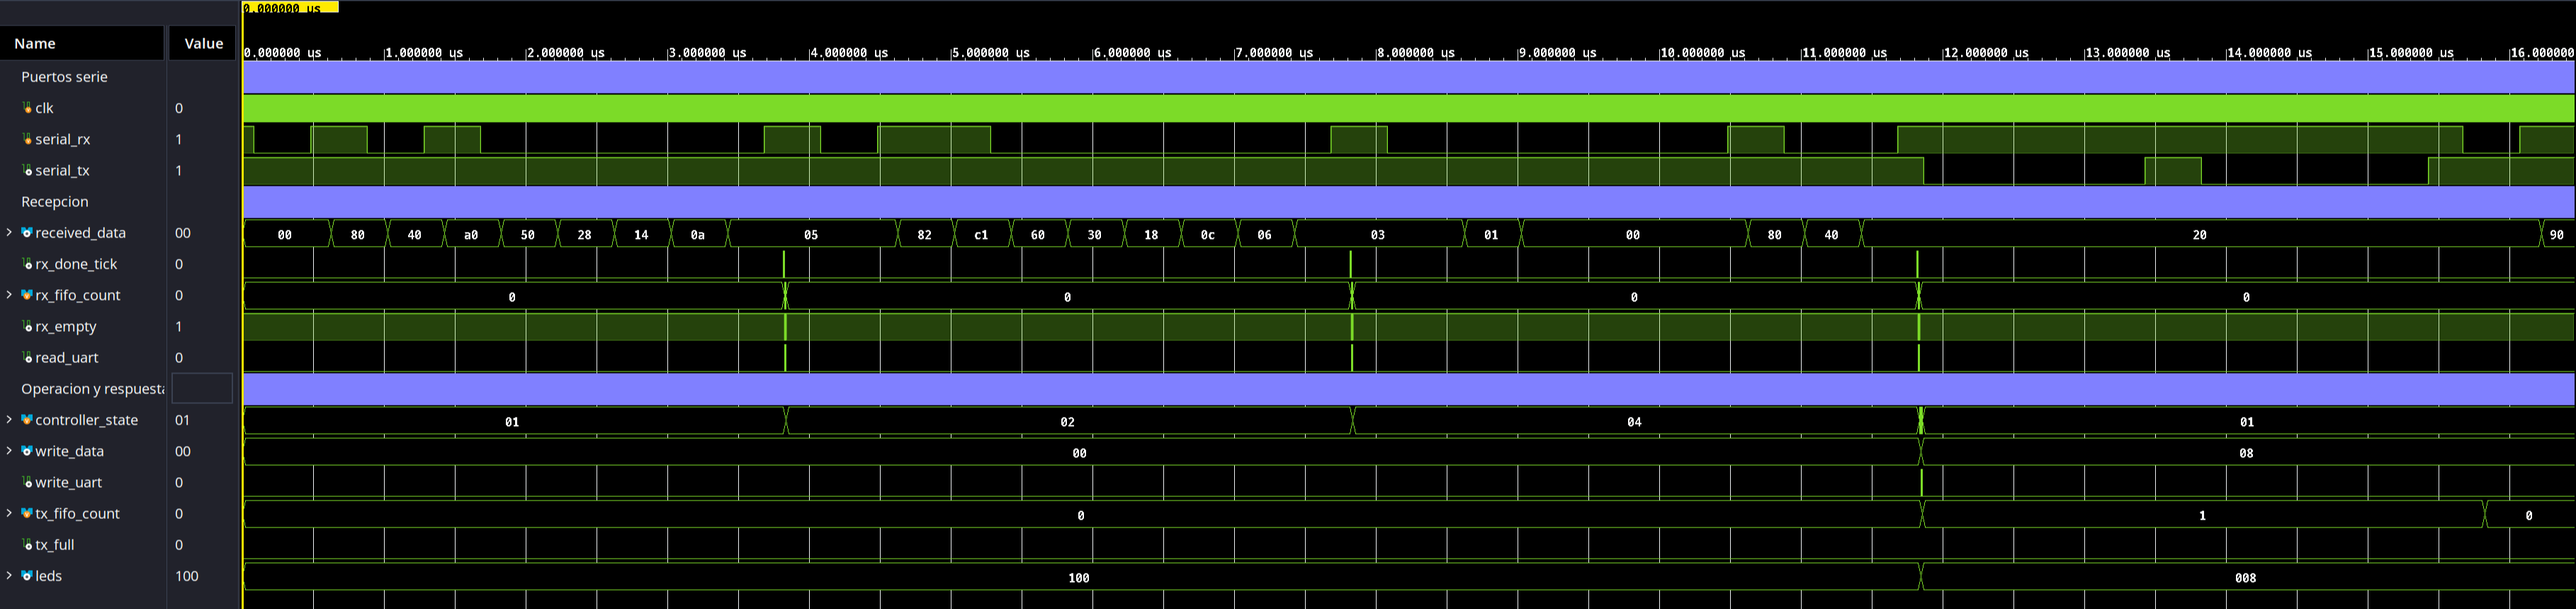
\includegraphics[width=\textwidth]{img/vivado_wave_top_end_to_end.png}
	\caption{Recorrido completo de \texttt{05 03 20} en
	\texttt{alu\_uart\_top\_tb}.}%
	\label{fig:wave-top-end-to-end}
\end{figure}

La regresión completa se compiló y ejecutó nuevamente mediante el archivo
\texttt{scripts/run\allowbreak\_tests.sh} con XSim 2025.2. La
figura~\ref{fig:regresion-xsim} reúne las líneas finales emitidas por los ocho
bancos. El registro completo de la ejecución se conserva en
\texttt{reports/simulation\allowbreak\_regression.log}.

El banco superior finalizó con
\texttt{PASS: 812 complete serial ALU transactions}. Después de ejecutar los
ocho bancos, el script informó
\texttt{PASS: 8 testbenches completados}.

\begin{figure}[H]
	\centering
	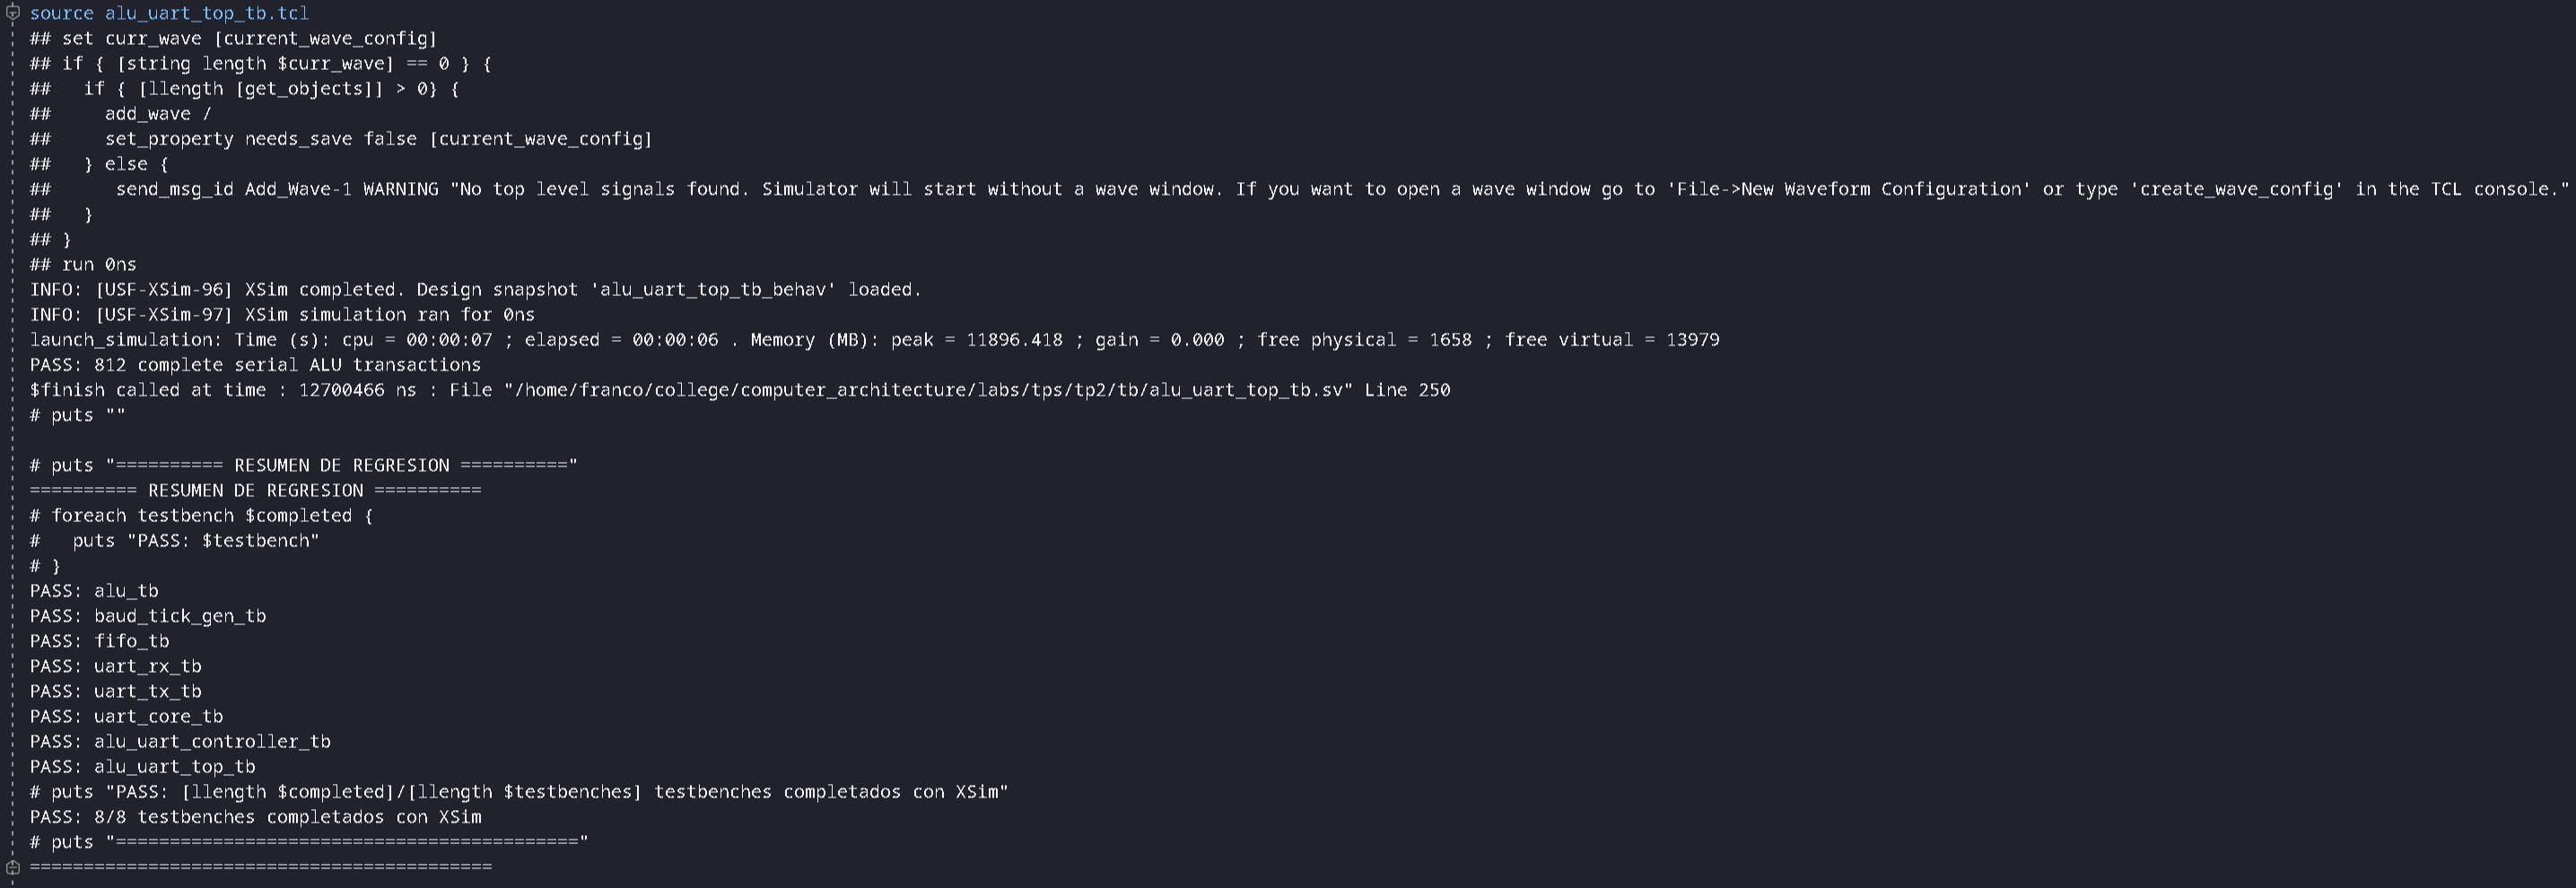
\includegraphics[width=\textwidth]{img/vivado_simulation_regression.png}
	\caption{Resultado de la regresión completa ejecutada con XSim 2025.2.}%
	\label{fig:regresion-xsim}
\end{figure}

\begin{table}[H]
	\centering
	\begin{tabularx}{\textwidth}{L{5.1cm}C{2.2cm}Y}
		\toprule
		\textbf{Banco} & \textbf{Estado} & \textbf{Resultado principal} \\
		\midrule
		\texttt{alu\_tb} & PASS & 814 comprobaciones. \\
		\texttt{baud\_tick\_gen\_tb} & PASS & Tick cada diez ciclos. \\
		\texttt{fifo\_tb} & PASS & Fronteras y wrap-around. \\
		\texttt{uart\_rx\_tb} & PASS & Tramas válidas y defectuosas. \\
		\texttt{uart\_tx\_tb} & PASS & Framing, orden y tiempos. \\
		\texttt{uart\_core\_tb} & PASS & FIFO, overrun y salida serie. \\
		\texttt{alu\_uart\_controller\_tb} & PASS & Protocolo y recuperación. \\
		\texttt{alu\_uart\_top\_tb} & PASS & 812 transacciones completas. \\
		\bottomrule
	\end{tabularx}
	\caption{Resultado de la regresión RTL completa.}%
\end{table}

\subsection{Interpretación}

El banco superior comprobó el recorrido funcional desde el pin RX hasta el pin
TX. La prueba incluyó el orden de los bits, el almacenamiento de los bytes, la
ejecución de la ALU, la transmisión de la respuesta y la permanencia del
resultado en los LED.

Los casos de recuperación confirmaron que el timeout, el bit de stop inválido y
el reset no producen una respuesta espuria. Después de cada situación, una
transacción nueva pudo completarse correctamente. Las 800 operaciones
aleatorias ampliaron la cantidad de operandos ejercitados mediante una
secuencia que puede repetirse con la misma semilla.

Estos resultados comprueban el comportamiento funcional del RTL, pero no
representan todos los fenómenos presentes en el circuito físico. La simulación
no modela la metastabilidad analógica ni el ruido de las señales. Tampoco
incluye la tolerancia de los osciladores, las demoras del enlace USB ni los
retardos obtenidos después del ruteo.

El análisis CDC y la verificación temporal del diseño implementado consideran
parte de estos aspectos en las secciones siguientes. La comunicación con el
puente USB--UART y la observación de los LED requieren una comprobación
posterior sobre la placa.
